\chapter{Существующие алгоритмы} \label{ch:ch2}

\section{Анализ} \label{sec:ch2/sec1}

В основном в качестве источника информации используются статьи \cite{dai, hodge, vakili, varun, billor, wilkinson}

\section{Основы алгоритмов} \label{sec:ch2/sec1}

Задачу поиска аномалий можно отнести к классу задач обучения без учителя. Суть поиска аномалий заключается в том, чтобы найти в выборке объекты, которые не похожи на большинство объектов выборки, т. е. те, которые выделяются на фоне других.

Часто бывает так, что аномальных объектов либо нет вообще, либо их очень мало и неизвестно где именно в выборке они находятся. Поэтому поиск аномалий относится к классу задач обучения без учителя (т. к. отсутствуют размеченные данные).

\section{Подходы к решению} \label{sec:ch2/sec2}

Одним из возможных способов определения аномалий является измерение схожести между объектов. У такого способа есть два варианта:
\begin{enumerate}
  \item Восстановление плотности
  \item Классификация
\end{enumerate}

\subsection{Восстановление плотности}

В случае с восстановлением плотности необходимо построить распределение, которое хорошо описывает выборку. И это распределение позволяет посчитать вероятность для нового объекта получить его из распределения, описывающего выборку.

В терминах этого метода аномалия - объект, полученный из другого распределения, описывающего другую выборку данных.

Есть три подхода:
\begin{enumerate}
  \item Параметрический
  \item Непараметрический
  \item Восстановление смесей
\end{enumerate}

\textbf{Параметрический метод}

Распределение представляется в виде $p(x)=\phi(x\vert\theta)$, где $\theta$ выступает в качестве параметра распределения. Например, в семейство параметрических распределений входит распределение Гаусса - $\theta=(\mu, \Sigma)$, где $\mu$ - вектор средних и $\Sigma$ - ковариационная матрица.

Параметры модели подбираются таким образом, чтобы вероятность объектов из обучающей выборки была максимальной. Для этого обычно пользуются Методом Максимального Правдоподобия:

\[ \sum_{i}\log\phi(x_{i}\vert\theta) \rightarrow \max_{\theta} \]

%\begin{figure}[ht]
%  \centering
%  
\includegraphics [scale=0.27] {latex}
%  \caption{TeX.}
%  \label{fig:latex}
%\end{figure}
%
%\section{Длинное название параграфа, в котором мы узнаём как сделать две картинки с~общим номером и названием} \label{sec:ch2/sect2}
%
%А это две картинки под общим номером и названием:
%\begin{figure}[ht]
%  \begin{minipage}[ht]{0.49\linewidth}\centering
%    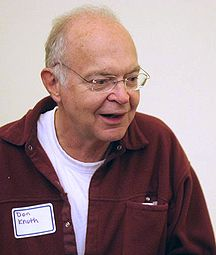
\includegraphics[width=0.5\linewidth]{knuth1} \\ а)
%  \end{minipage}
%  \hfill
%  \begin{minipage}[ht]{0.49\linewidth}\centering
%    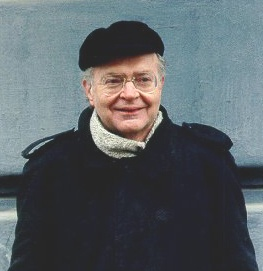
\includegraphics[width=0.5\linewidth]{knuth2} \\ б)
%  \end{minipage}
%  \caption{Очень длинная подпись к изображению,
%      на котором представлены две фотографии Дональда Кнута}
%  \label{fig:knuth}
%\end{figure}
%
%Те~же~две картинки под~общим номером и~названием,
%но с автоматизированной нумерацией подрисунков:
%\begin{figure}[ht]
%    {\centering
%        \hfill
%        \subbottom[List-of-Figures entry][Первый подрисунок\label{fig:knuth_2-1}]{%
%            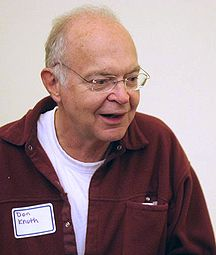
\includegraphics[width=0.25\linewidth]{knuth1}}
%        \hfill
%        \subbottom[\label{fig:knuth_2-2}]{%
%            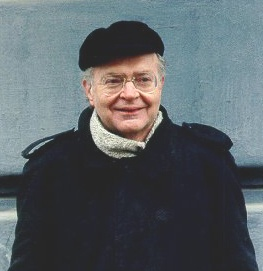
\includegraphics[width=0.25\linewidth]{knuth2}}
%        \hfill
%        \subbottom[Третий подрисунок]{%
%            \includegraphics[width=0.3\linewidth]{example-image-c}}
%        \hfill
%    }
%    \legend{Подрисуночный текст, описывающий обозначения, например. Согласно
%    ГОСТ 2.105, пункт 4.3.1, располагается перед наименованием рисунка.}
%    \caption[Этот текст попадает в названия рисунков в списке рисунков]{Очень
%    длинная подпись к второму изображению, на~котором представлены две
%    фотографии Дональда Кнута}
%    \label{fig:knuth_2}
%\end{figure}
%
%На рисунке~\ref{fig:knuth_2-1} показан Дональд Кнут без головного убора.
%На рисунке~\ref{fig:knuth_2}\subcaptionref*{fig:knuth_2-2}
%показан Дональд Кнут в головном уборе.
%
%Возможно вставлять векторные картинки, рассчитываемые \LaTeX\ <<на~лету>>
%с~их~предварительной компиляцией. Надписи в таких рисунках будут выполнены
%тем же~шрифтом, который указан для документа в целом.
%На~рисунке~\ref{fig:tikz_example} на~странице~\pageref{fig:tikz_example}
%представлен пример схемы, рассчитываемой пакетом \verb|tikz| <<на~лету>>.
%Для ускорения компиляции, подобные рисунки могут быть <<кешированы>>, что
%определяется настройками в~\verb|common/setup.tex|.
%Причём имя предкомпилированного
%файла и~папка расположения таких файлов могут быть отдельно заданы,
%что удобно, если не~для подготовки диссертации,
%то~для подготовки научных публикаций.
%\begin{figure}[ht]
%    \legend{}
%    \caption[Пример \texttt{tikz} схемы]{Пример рисунка, рассчитываемого
%        \texttt{tikz}, который может быть предкомпилирован}
%    \label{fig:tikz_example}
%\end{figure}
%
%Множество программ имеют либо встроенную возможность экспортировать векторную
%графику кодом \verb|tikz|, либо соответствующий пакет расширения.
%Например, в GeoGebra есть встроенный экспорт,
%для Inkscape есть пакет svg2tikz,
%для Python есть пакет matplotlib2tikz,
%для R есть пакет tikzdevice.